% =====================================================================
%  The Mathematics of HATI -- a complete derivation
%  from a single pixel to a learned hazard probability
%  Author: Gergő Csaba Morvai
%  Engine: LuaLaTeX   (compile: latexmk -lualatex hati_math.tex)
% =====================================================================
\documentclass[11pt]{article}

\usepackage{fontspec}
\usepackage{microtype}
\usepackage[a4paper,margin=2.2cm]{geometry}
\usepackage{amsmath,amssymb,amsthm,mathtools}
\usepackage{siunitx}
\sisetup{detect-all}
\usepackage{xcolor}
\usepackage{tikz}
\usetikzlibrary{positioning,arrows.meta,calc,decorations.pathmorphing}
\usepackage{tcolorbox}
\tcbuselibrary{skins,breakable}
\usepackage{titlesec}
\usepackage{enumitem}
\usepackage[hidelinks]{hyperref}

\setmainfont{TeX Gyre Pagella}
\setsansfont{TeX Gyre Heros}[Scale=0.92]
\setmonofont{TeX Gyre Cursor}[Scale=0.9]

\allowdisplaybreaks

% ---- palette ----
\definecolor{hb}{HTML}{1F3A5F}
\definecolor{ha}{HTML}{B23A2E}
\definecolor{hg}{HTML}{1B7A6E}
\definecolor{wbg}{HTML}{EAF2FB}
\definecolor{wfr}{HTML}{2E6DB4}

\titleformat{\section}{\sffamily\large\bfseries\color{hb}}{\thesection}{0.6em}{}
\titleformat{\subsection}{\sffamily\normalsize\bfseries\color{hb!88}}{\thesubsection}{0.5em}{}

% ---- "in words" explanation box ----
\newtcolorbox{words}{breakable,enhanced,colback=wbg,colframe=wfr,boxrule=0.5pt,
  arc=2pt,left=7pt,right=7pt,top=4pt,bottom=4pt,
  fonttitle=\bfseries\sffamily\small,coltitle=wfr,
  attach boxed title to top left={xshift=8pt,yshift=-7pt},
  boxed title style={colback=wbg,colframe=wfr,boxrule=0.4pt,arc=1pt},
  title={In words}}

% ---- theorem environments ----
\theoremstyle{definition}
\newtheorem{definition}{Definition}[section]
\newtheorem{proposition}{Proposition}[section]
\newtheorem{remark}{Remark}[section]

% ---- math macros ----
\newcommand{\R}{\mathbb{R}}
\newcommand{\Z}{\mathbb{Z}}
\newcommand{\Ex}{\mathbb{E}}
\newcommand{\grad}{\nabla}
\newcommand{\lap}{\nabla^2}
\newcommand{\norm}[1]{\left\lVert #1 \right\rVert}
\newcommand{\abs}[1]{\left\lvert #1 \right\rvert}
\newcommand{\set}[1]{\left\{ #1 \right\}}
\newcommand{\med}{\operatorname{med}}
\newcommand{\IQR}{\operatorname{IQR}}
\newcommand{\clip}{\operatorname{clip}}
\newcommand{\sgn}{\operatorname{sgn}}
\newcommand{\diag}{\operatorname{diag}}
\newcommand{\T}{^{\mathsf{T}}}
\newcommand{\conv}{\mathbin{\ast}}
\newcommand{\half}{\tfrac{1}{2}}
\DeclareMathOperator*{\argmin}{arg\,min}

\title{\sffamily\bfseries\color{hb}\Large The Mathematics of \textsc{Hati}\\[2pt]
\large A complete derivation: from a single pixel to a learned hazard probability}
\author{\normalsize Gerg\H{o} Csaba Morvai \\[2pt]
\footnotesize\itshape HATI v2.0 \textendash{} M\'ani Mission terrain-hazard pipeline}
\date{\footnotesize\today}

\begin{document}
\maketitle

\begin{abstract}\noindent
This document derives, from first principles and in full, the mathematics behind
\textsc{Hati}'s two terrain-hazard channels. We start with one pixel and a number
attached to it, build the discrete differential geometry that turns an elevation
grid into ten roughness fields, derive the robust statistics that put those fields
on a common footing, and show that the fusion step is exactly a logistic
generalized linear model --- the same object as a one-neuron classifier. We then
develop the full machine-learning apparatus that would \emph{learn} that model
(likelihood, cross-entropy, the gradient, the Hessian, regularization, and the
backpropagation identity), the exact additive attribution that makes the score
interpretable, the projective geometry that places a selenographic coordinate on a
pixel, the ray geometry of a cast shadow, the second-moment ellipse algebra of the
shadow census, and the sampling theorem that defines the resolution floor both
channels are built around. Every block of algebra is followed by a plain-language
unpacking. The aim is a single, self-contained derivation you could write across a
blackboard and, having understood it, hold the whole pipeline in your head.
\end{abstract}

\begin{center}\small\itshape
Read it once for the shape, once for the algebra, once for the meaning.
\end{center}

\tableofcontents
\bigskip

% =====================================================================
\section{The object of study: a discrete field on a lattice}

\begin{definition}[Digital elevation model]
Let $\Omega = \set{0,\dots,M-1}\times\set{0,\dots,N-1}\subset\Z^2$ be a finite
pixel lattice. A \emph{digital elevation model} (DEM) is a map
\[
z:\Omega\longrightarrow \R\cup\set{\varnothing},\qquad (i,j)\mapsto z_{ij},
\]
assigning to each pixel a height in metres, or the symbol $\varnothing$ (no data).
Each pixel covers a square of side $s$ metres on the ground; $s$ is the
\emph{ground sample distance}. The set of valid pixels is
$\Omega^\star=\set{(i,j)\in\Omega: z_{ij}\neq\varnothing}$.
\end{definition}

\begin{definition}[Affine geotransform]
The lattice is tied to projected ground coordinates $(X,Y)\in\R^2$ (metres) by an
affine map
\begin{equation}
\begin{pmatrix}X\\Y\end{pmatrix}
=\begin{pmatrix}X_0\\Y_0\end{pmatrix}
+\begin{pmatrix} s & 0\\ 0 & -s\end{pmatrix}
\begin{pmatrix} j \\ i\end{pmatrix},
\label{eq:geo}
\end{equation}
where $(X_0,Y_0)$ is the upper-left corner, column $j$ runs east, row $i$ runs
south. The matrix is the \emph{geotransform} $G$; it is invertible whenever
$s\neq0$, with $G^{-1}$ recovering $(j,i)$ from $(X,Y)$.
\end{definition}

\begin{words}
A DEM is just a grid of numbers: at row $i$, column $j$, the ground is $z_{ij}$
metres high. Each cell is $s$ metres across (for our lunar map, $s=\SI{4}{m}$).
Equation~\eqref{eq:geo} is the dictionary between ``which cell'' and ``where on the
Moon, in metres.'' Everything \textsc{Hati} does to the terrain is an operation on
this grid of numbers; everything that places it on the Moon is this affine map and
the projection of the next section.
\end{words}

% =====================================================================
\section{Map I: from a selenographic coordinate to a pixel}

The touchdown is given as latitude $\varphi$ and longitude $\lambda$ on a sphere of
radius $R=\SI{1737.4}{km}$. We need its pixel. The bridge is the
\emph{south-polar stereographic projection}.

\subsection{Deriving the stereographic projection}

Place the sphere with its south pole $S$ tangent to a plane $\Pi$, and project every
surface point $P$ from the north pole $N$ through $P$ onto $\Pi$. Let $\theta$ be the
angular distance of $P$ from $S$ (the colatitude measured from the south pole). In
the plane through $N$, $S$, $P$, the inscribed-angle relation gives the projected
radius
\begin{equation}
\rho(\theta) = 2R\tan\!\left(\frac{\theta}{2}\right).
\label{eq:rho}
\end{equation}
Latitude relates to this colatitude by $\theta = \tfrac{\pi}{2}+\varphi$ (at $S$,
$\varphi=-\tfrac{\pi}{2}\Rightarrow\theta=0$; at the equator $\varphi=0\Rightarrow
\theta=\tfrac{\pi}{2}$). Substituting,
\begin{equation}
\boxed{\;\rho(\varphi) = 2R\tan\!\left(\frac{\pi}{4}+\frac{\varphi}{2}\right),\qquad
X = \rho\sin\lambda,\quad Y=\rho\cos\lambda.\;}
\label{eq:stereo}
\end{equation}

\begin{proposition}[Conformality and the point scale]
The map \eqref{eq:stereo} is conformal (angle-preserving), and its isotropic point
scale factor is
\begin{equation}
m(\varphi)=\frac{d\rho}{R\,d\theta}=\sec^2\!\left(\frac{\theta}{2}\right)
=\sec^2\!\left(\frac{\pi}{4}+\frac{\varphi}{2}\right).
\label{eq:scale}
\end{equation}
\end{proposition}
\begin{proof}
Differentiate \eqref{eq:rho}: $\dfrac{d\rho}{d\theta}=2R\cdot\half\sec^2(\theta/2)
=R\sec^2(\theta/2)$. The meridian arc element on the sphere is $R\,d\theta$, so the
radial scale is $\sec^2(\theta/2)$. The parallel (circumferential) scale is
$\rho/(R\sin\theta)$; using $\rho=2R\tan(\theta/2)$ and
$\sin\theta=2\sin(\theta/2)\cos(\theta/2)$ gives the same $\sec^2(\theta/2)$. Equal
radial and circumferential scales $\Rightarrow$ conformal, with common factor
\eqref{eq:scale}. At the pole $\theta=0$, $m=1$: true scale.
\end{proof}

Finally, compose with the inverse geotransform: the pixel of the touchdown is
\begin{equation}
\begin{pmatrix}j^\star\\ i^\star\end{pmatrix}
=\left\lfloor G^{-1}\!\begin{pmatrix}\rho(\varphi)\sin\lambda\\ \rho(\varphi)\cos\lambda\end{pmatrix}\right\rceil ,
\label{eq:tdpixel}
\end{equation}
$\lfloor\cdot\rceil$ rounding to the nearest integer lattice point.

\begin{words}
To find which pixel a latitude/longitude lands on, imagine standing at the north
pole and shining every south-polar point onto a flat sheet under the south pole.
A point's distance from the centre, $\rho$, depends only on its latitude
(Eq.~\ref{eq:stereo}); the direction is its longitude. Near the pole the map barely
distorts anything --- that is what $m\to1$ in Eq.~\eqref{eq:scale} means --- so a
metre on our map is a metre on the Moon. Equation~\eqref{eq:tdpixel} then just reads
off the row and column.
\end{words}

% =====================================================================
\section{Differential operators on the pixel lattice}

All of Channel~1 is built from two differential primitives --- the gradient and the
Laplacian --- realised as \emph{convolutions} of the grid with small kernels.

\begin{definition}[Discrete convolution]
For a kernel $K\in\R^{(2r+1)\times(2r+1)}$ and field $f:\Omega\to\R$,
\begin{equation}
(K\conv f)_{ij}=\sum_{a=-r}^{r}\sum_{b=-r}^{r}K_{ab}\,f_{i-a,\,j-b}.
\end{equation}
\end{definition}

The first derivatives use central differences (here the Sobel kernels, which average
over three rows/columns for noise tolerance):
\begin{equation}
\partial_X z \approx \frac{1}{8s}\,(K_x\conv z),\quad
\partial_Y z \approx \frac{1}{8s}\,(K_y\conv z),\quad
K_x=\begin{psmallmatrix}-1&0&1\\-2&0&2\\-1&0&1\end{psmallmatrix},\;
K_y=\begin{psmallmatrix}-1&-2&-1\\0&0&0\\1&2&1\end{psmallmatrix}.
\end{equation}
The factor $1/s$ converts ``per pixel'' to ``per metre.'' The \emph{slope field} is the
magnitude of the gradient, returned as an angle:
\begin{equation}
\boxed{\;\sigma_{ij}=\arctan\sqrt{(\partial_X z)_{ij}^2+(\partial_Y z)_{ij}^2}\;}\qquad\in[0,\tfrac{\pi}{2}).
\label{eq:slope}
\end{equation}
The second derivative (curvature) uses the five-point Laplacian stencil:
\begin{equation}
(\lap z)_{ij}\approx\frac{1}{s^2}\,(K_L\conv z)_{ij},\qquad
K_L=\begin{psmallmatrix}0&1&0\\1&-4&1\\0&1&0\end{psmallmatrix}.
\label{eq:lap}
\end{equation}

\begin{words}
``Slope'' is rise-over-run, measured by comparing each pixel to its neighbours
(that's all a Sobel kernel does --- a weighted left-minus-right and up-minus-down).
Take the steepness in both directions, combine by Pythagoras, and report the angle:
Eq.~\eqref{eq:slope}. ``Curvature'' (Eq.~\ref{eq:lap}) compares a pixel to the
average of its four neighbours: positive in a bowl, negative on a dome, zero on a
flat or evenly-tilted patch. These two numbers, slope and curvature, are the atoms
everything else is built from.
\end{words}

% =====================================================================
\section{Windowed and order statistics}

Roughness is not a per-pixel quantity; it lives in a \emph{neighbourhood}. Let
$\mathcal{W}_{ij}$ be the $w\times w$ window centred on $(i,j)$, with
$n=w^2$ pixels.

\paragraph{Moment statistics (via the box kernel).} With the uniform kernel
$U=\frac{1}{n}\mathbf{1}_{w\times w}$, the windowed mean and mean-square of a field
$f$ are $\mu_f=U\conv f$ and $\overline{f^2}=U\conv f^2$, so the windowed RMS and
variance are
\begin{equation}
\operatorname{RMS}_w f=\sqrt{U\conv f^2},\qquad
\operatorname{Var}_w f=(U\conv f^2)-(U\conv f)^2 .
\label{eq:rms}
\end{equation}

\paragraph{Order statistics.} Sort the $n$ window values
$f^{(1)}\le f^{(2)}\le\dots\le f^{(n)}$. The $p$-quantile is
$Q_p(f)_{ij}=f^{(\lceil pn\rceil)}$, and the interquartile range is
\begin{equation}
\IQR_w f = Q_{0.75}(f)-Q_{0.25}(f).
\label{eq:iqr}
\end{equation}
The median is $\med_w f=Q_{0.5}(f)$. Order statistics are nonlinear --- not
convolutions --- which is exactly why they resist outliers.

\begin{words}
A single pixel can't be ``rough.'' So we slide a little square window over the map
and, at each position, summarise the values inside it. Two kinds of summary: moments
(mean, RMS, variance --- which we get cheaply as box-blurs, Eq.~\ref{eq:rms}) and
order statistics (median, quartiles, IQR --- which need sorting, Eq.~\ref{eq:iqr}).
The order statistics are the robust ones: a single freak value can't drag a median
the way it drags a mean.
\end{words}

% =====================================================================
\section{The ten Tier-1 channels}

We now define every channel as an operator $C_k[z]:\Omega\to\R_{\ge0}$ on the DEM.
Write $\sigma=\sigma[z]$ for the slope field~\eqref{eq:slope} and $\ell=\lap z$ for
the Laplacian~\eqref{eq:lap}.

\begin{align}
\text{RMS slope:}&& C_1 &= \sqrt{U\conv \sigma^2}, \\
\text{Slope IQR:}&& C_2 &= \IQR_w\,\sigma, \\
\text{Curvature IQR:}&& C_3 &= \IQR_w\,\ell, \\
\text{Planar deviation:}&& C_4 &= \sqrt{U\conv(z-U\conv z)^2}, \\
\text{$\lvert$TPI$\rvert$:}&& C_5 &= \abs{\,z-U\conv z\,}, \\
\text{TRI:}&& C_6 &= \tfrac{1}{8}\!\!\sum_{(a,b)\in\mathcal{N}_8}\!\!\abs{z-S_{ab}z}, \\
\text{MDS at scale }L:&& C_{7\dots10} &= \med_w\Big|\,\sigma[G_{\sigma_L}\!\conv z]-\sigma[G_{\sigma_{2L}}\!\conv z]\,\Big|,
\end{align}
where $S_{ab}z$ is the shift of $z$ by $(a,b)$, $\mathcal{N}_8$ the eight neighbours,
and $G_{\sigma}$ the Gaussian kernel $G_\sigma(a,b)=\frac{1}{2\pi\sigma^2}
e^{-(a^2+b^2)/2\sigma^2}$ with smoothing radius $\sigma_L = L/3$. The four MDS
channels use $L\in\set{2,3,5,8}$ px, i.e.\ $\set{8,12,20,32}\,\si{m}$.

\begin{words}
Each channel is one ``flavour of rough,'' all built from slope and curvature inside
the sliding window:
\emph{RMS slope} = how steep on average; \emph{Slope IQR} = how much the slope
\emph{varies in direction} (a crater field scatters slopes every way); \emph{Curvature
IQR} = spread of bowl-vs-dome (the crater signature); \emph{Planar deviation} = how
bumpy relative to a local flat fit; \emph{$|$TPI$|$} = how far a point sits above or
below its surroundings (rim or pit); \emph{TRI} = jaggedness to immediate neighbours;
\emph{MDS} = the clever one --- blur to size $L$ and to size $2L$, subtract the
slopes, and what survives is the roughness living \emph{specifically} at size $L$.
Run it at four sizes and you get a little spectrum of bumpiness across
$8$--$\SI{32}{m}$, bracketing the crater that mattered.
\end{words}

% =====================================================================
\section{Robust normalization: putting ten channels on one ruler}

The ten fields have different units and wildly different scales. Before combining
them we standardise each one against \emph{its own distribution on the scene}.

\paragraph{Tail compression.} Roughness fields are non-negative and long-tailed, so
we first apply $g(x)=\log(1+x)$, which is monotone (preserves ranking) and squashes
the tail.

\paragraph{Robust location and scale.} Instead of mean and standard deviation
(which the tail corrupts) we use the median and the IQR. The scale estimate is
$\hat s = \IQR/1.349$, and the standardised, clipped channel is
\begin{equation}
\boxed{\;\zeta_k = \clip_{\pm c}\!\left(\frac{g(C_k)-\med\big(g(C_k)\big)}{\IQR\big(g(C_k)\big)/1.349}\right),\quad
\clip_{\pm c}(t)=\max(-c,\min(c,t)),\ c=4.\;}
\label{eq:zscore}
\end{equation}

\begin{proposition}[Why $1.349$]
If $C\sim\mathcal N(\mu,s^2)$, then $\IQR(C)=1.349\,s$, so $\IQR/1.349$ is a
consistent estimator of $s$.
\end{proposition}
\begin{proof}
For the standard normal with CDF $\Phi$, the quartiles are $\pm\Phi^{-1}(0.75)$.
Numerically $\Phi^{-1}(0.75)=0.674489\ldots$, so for $\mathcal N(\mu,s^2)$,
\[
\IQR = s\big(\Phi^{-1}(0.75)-\Phi^{-1}(0.25)\big)=s\cdot 2(0.674489)=1.34898\,s.
\]
Dividing by $1.349$ inverts this, recovering $s$. \qedhere
\end{proof}

\begin{words}
Each roughness map is centred (subtract its typical value) and rescaled (divide by
its typical spread), so a value of ``$+2$'' means the same thing --- two spreads
above normal --- in every channel. We use the median and IQR rather than mean and
standard deviation so a handful of extreme pixels can't define ``normal.'' The
mysterious $1.349$ is just the width, in IQRs, of a bell curve (Proposition~6.1):
dividing by it turns an IQR back into an ordinary standard deviation. The clip at
$\pm4$ stops any one pixel from screaming over the rest.
\end{words}

% =====================================================================
\section{The fusion is a generalized linear model}

Collect the ten standardised channels at a pixel into a \emph{feature vector}
$\boldsymbol\zeta(x)=\big(\zeta_1(x),\dots,\zeta_{10}(x)\big)\T\in\R^{10}$, with a
literature weight vector $\mathbf w\in\R^{10}$ and bias $b$. \textsc{Hati}'s hazard
score is
\begin{equation}
\boxed{\;H(x)=\sigma\!\Big(\underbrace{\tfrac{1}{\norm{\mathbf w}_1}\,\mathbf w\T\boldsymbol\zeta(x)+b}_{\textstyle a(x)\ \text{(pre-activation)}}\Big),\qquad
\sigma(a)=\frac{1}{1+e^{-a}},\quad b=-1.\;}
\label{eq:fuse}
\end{equation}
This is \emph{exactly} a logistic-regression unit / a single sigmoidal neuron:
$\norm{\mathbf w}_1=\sum_k\abs{w_k}$ normalises so the output midpoint does not drift
with the number of channels. The per-pixel hazard is therefore a point on the
logistic curve, driven by a weighted vote of the ten standardised roughness fields.

\paragraph{Exact additive attribution.} Because the pre-activation is linear, the
score decomposes \emph{exactly} into per-channel contributions
\begin{equation}
a(x)=b+\sum_{k=1}^{10}\phi_k(x),\qquad \phi_k(x)=\frac{w_k\,\zeta_k(x)}{\norm{\mathbf w}_1},
\label{eq:attr}
\end{equation}
so ``why did this pixel score high?'' has a closed-form answer: read off the
$\phi_k$. For a linear model this coincides with the Shapley value
$\phi_k^{\text{Sh}}=\frac{w_k}{\norm{\mathbf w}_1}\big(\zeta_k-\Ex[\zeta_k]\big)$ up to
the constant baseline --- attribution is not an approximation here, it is the model.

\begin{words}
Here is the heart of it. Stack the ten normalised roughness numbers for a pixel into
a vector. Multiply by a weight vector (how much each one matters), add them, add a
bias, and squash the total through an S-curve into a probability between 0 and 1.
That S-curve squashing of a weighted sum \emph{is} the simplest possible classifier
--- one artificial neuron. And because the inside is just a sum
(Eq.~\ref{eq:attr}), you can always say exactly how much each channel pushed the
score, which is why \textsc{Hati} is interpretable where a deep network is a black
box.
\end{words}

% =====================================================================
\section{The machine learning: learning the weights}

\textsc{Hati} fixes $\mathbf w$ from the literature. The natural generalization is to
\emph{learn} it from labelled terrain. This section is the full apparatus.

\subsection{The model as a probability}
Treat the label $y\in\set{0,1}$ (safe / hazardous) as Bernoulli with
$\Pr(y=1\mid x)=H(x)=\sigma(\mathbf w\T\boldsymbol\zeta+b)$. Absorb $b$ into
$\mathbf w$ by appending a constant feature. Over a dataset
$\set{(\boldsymbol\zeta^{(m)},y^{(m)})}_{m=1}^{D}$ the likelihood is
\begin{equation}
\mathcal L(\mathbf w)=\prod_{m=1}^{D} H_m^{\,y^{(m)}}\,(1-H_m)^{\,1-y^{(m)}},\qquad H_m=\sigma(\mathbf w\T\boldsymbol\zeta^{(m)}).
\end{equation}

\subsection{The loss and its gradient}
Maximising likelihood $=$ minimising the negative log-likelihood, the
\emph{binary cross-entropy}:
\begin{equation}
J(\mathbf w)=-\frac{1}{D}\sum_{m=1}^{D}\Big[y^{(m)}\log H_m+(1-y^{(m)})\log(1-H_m)\Big].
\label{eq:bce}
\end{equation}
Using the clean identity $\sigma'(a)=\sigma(a)\big(1-\sigma(a)\big)$, the gradient
collapses beautifully:
\begin{align}
\frac{\partial J}{\partial \mathbf w}
&=-\frac1D\sum_m\left[\frac{y^{(m)}}{H_m}-\frac{1-y^{(m)}}{1-H_m}\right]\sigma'(a_m)\,\boldsymbol\zeta^{(m)}\notag\\
&=-\frac1D\sum_m\left[\frac{y^{(m)}-H_m}{H_m(1-H_m)}\right]H_m(1-H_m)\,\boldsymbol\zeta^{(m)}
=\boxed{\;\frac{1}{D}\sum_{m=1}^{D}\big(H_m-y^{(m)}\big)\,\boldsymbol\zeta^{(m)}.\;}
\label{eq:grad}
\end{align}
Gradient descent then iterates $\mathbf w \leftarrow \mathbf w-\eta\,\partial_{\mathbf w}J$
with learning rate $\eta$.

\subsection{Curvature: the Hessian and Newton's method}
Differentiating \eqref{eq:grad} again,
\begin{equation}
\mathbf H=\frac{\partial^2 J}{\partial\mathbf w\,\partial\mathbf w\T}
=\frac{1}{D}\sum_m H_m(1-H_m)\,\boldsymbol\zeta^{(m)}\boldsymbol\zeta^{(m)\mathsf T}
=\frac1D\,\Phi\T S\,\Phi\succeq 0,
\label{eq:hess}
\end{equation}
with design matrix $\Phi=[\boldsymbol\zeta^{(1)}\!,\dots]\T$ and
$S=\diag\big(H_m(1-H_m)\big)$. Positive semi-definiteness proves $J$ is
\emph{convex}: no spurious local minima. Newton's method (here, iteratively
reweighted least squares) updates $\mathbf w\leftarrow\mathbf w-\mathbf H^{-1}\partial_{\mathbf w}J$.

\subsection{Regularization}
A zero-mean Gaussian prior $\mathbf w\sim\mathcal N(0,\tau^2 I)$ turns maximum
likelihood into maximum-a-posteriori, adding the ridge penalty
\begin{equation}
J_\lambda(\mathbf w)=J(\mathbf w)+\frac{\lambda}{2}\norm{\mathbf w}_2^2,\qquad
\lambda=\frac{1}{D\tau^2},
\end{equation}
which keeps weights small (less overfitting) and makes $\mathbf H+\lambda I\succ0$
strictly --- a unique optimum.

\subsection{Backpropagation to a deeper model}
If the ten channels feed a hidden layer rather than a single neuron, write
$\mathbf h=\sigma(W^{[1]}\boldsymbol\zeta+\mathbf b^{[1]})$,
$H=\sigma(\mathbf w^{[2]\mathsf T}\mathbf h+b^{[2]})$. The chain rule (backprop)
propagates the error $\delta^{[2]}=H-y$ backward,
\begin{equation}
\delta^{[1]}=\big(\mathbf w^{[2]}\delta^{[2]}\big)\odot\mathbf h\odot(1-\mathbf h),\qquad
\frac{\partial J}{\partial W^{[1]}}=\delta^{[1]}\boldsymbol\zeta\T,
\end{equation}
$\odot$ the elementwise product --- the same $\sigma'=\sigma(1-\sigma)$ doing the
work at every layer. (For $k$ mutually-exclusive hazard classes one replaces
$\sigma$ by the softmax $\text{softmax}(a)_c=e^{a_c}/\sum_{c'}e^{a_{c'}}$ and the
loss by categorical cross-entropy; the gradient keeps the same $H-y$ form.)

\begin{words}
This is the part everyone calls ``training.'' Say which sites are safe ($y{=}0$) and
which are hazardous ($y{=}1$). The model guesses a probability $H$; the cross-entropy
(Eq.~\ref{eq:bce}) measures how wrong the guesses are. The miracle is
Eq.~\eqref{eq:grad}: the nudge each weight needs is just \emph{(prediction minus
truth) times the feature} --- push the weight up if you under-predicted hazard on a
rough feature, down if you over-predicted. Repeat. The Hessian
(Eq.~\ref{eq:hess}) being positive shows the problem is bowl-shaped --- one bottom,
no traps. Regularization keeps the weights modest; backprop is the same rule applied
layer by layer if you stack neurons. \textsc{Hati} currently \emph{skips} this step
and sets the weights from physics --- which is what makes it interpretable and
needs no training labels --- but this is the door to learning them.
\end{words}

% =====================================================================
\section{From a score field to a decision}

The hazard field $H:\Omega^\star\to(0,1)$ is \emph{relative}. To rank a point we use
the empirical cumulative distribution over valid pixels,
\begin{equation}
\widehat F_H(t)=\frac{1}{\abs{\Omega^\star}}\sum_{x\in\Omega^\star}\mathbf 1\!\set{H(x)\le t},
\end{equation}
and report the touchdown's percentile $\widehat F_H\!\big(H(x^\star)\big)$. As a unit-free
effect size we also give the robust $z$ against the median absolute deviation
$\mathrm{MAD}=\med_x\abs{H(x)-\med H}$,
\begin{equation}
z^\star=\frac{H(x^\star)-\med_x H}{1.4826\,\mathrm{MAD}},
\end{equation}
($1.4826=1/\Phi^{-1}(0.75)$ rescales MAD to a Gaussian $\sigma$). The decision rule
is $\text{flag}(x)=\mathbf 1\set{\widehat F_H(H(x))\ge\tau}$ for a chosen percentile
threshold $\tau$.

\begin{words}
A score of $0.73$ means nothing on its own --- is that bad? So we ask: \emph{what
fraction of the scene is less hazardous than this point?} That percentile is the
verdict. The robust $z$ says the same thing in ``how many spreads above typical.''
For the Athena touchdown both came out extreme (96th percentile, $z^\star=3.2$),
which is what ``flagged'' means.
\end{words}

% =====================================================================
\section{Channel 2: the geometry of a cast shadow}

The DEM stops at the pixel scale. Channel~2 reaches below it using shadows in a
finer photograph.

\subsection{Height from shadow length}
Let the Sun sit at elevation angle $e$ above the local horizon. An obstacle of height
$h$ blocks the grazing rays; the shadow it casts on flat ground has length $L$ where,
by the right triangle of ray, ground, and obstacle,
\begin{equation}
\tan e=\frac{h}{L}\quad\Longrightarrow\quad \boxed{\,h=L\tan e.\,}
\label{eq:relief}
\end{equation}
The shadow's \emph{width across} the Sun direction equals the obstacle's footprint and
is independent of $e$ (the Sun's elevation stretches the shadow only along its own
azimuth). So one shadow yields two numbers: an elevation-free footprint, and a height
that needs $e$.

\begin{center}
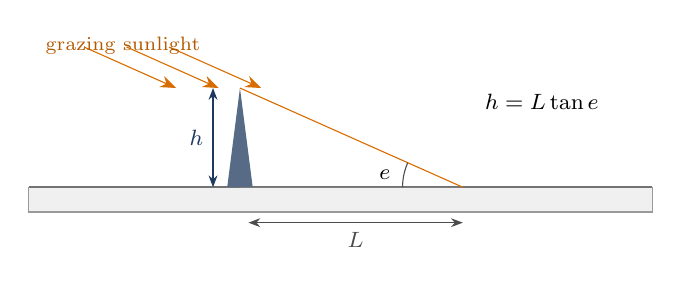
\begin{tikzpicture}[scale=0.9]
  \draw[fill=black!6,draw=black!40] (-0.2,0) rectangle (8.6,-0.35);
  \draw[thick,black!55] (-0.2,0)--(8.6,0);
  \def\hh{1.4}\pgfmathsetmacro{\LL}{\hh/tan(24)}
  \fill[hb!75] (2.6,0)--(2.78,\hh)--(2.96,0)--cycle;
  \coordinate(T) at (2.78,\hh);\coordinate(Sh) at ({2.78+\LL},0);
  \fill[black!22] (2.96,0)--(Sh)--(2.78,0)--cycle;
  \foreach \dx in {-0.9,-0.3,0.3}{\draw[-{Stealth[length=2mm]},orange!85!black]
     ($(T)+(\dx,0)+(-1.3,{1.3*tan(24)})$)--($(T)+(\dx,0)$);}
  \draw[orange!85!black] (T)--(Sh);
  \draw[black!70] (Sh)++(-0.85,0) arc (180:156:0.85);
  \node[font=\footnotesize] at ($(Sh)+(-1.1,0.18)$){$e$};
  \draw[{Stealth[length=1.5mm]}-{Stealth[length=1.5mm]},hb](2.4,0)--(2.4,\hh) node[midway,left,font=\footnotesize]{$h$};
  \draw[{Stealth[length=1.5mm]}-{Stealth[length=1.5mm]},black!70](2.9,-0.5)--($(Sh)+(0,-0.5)$) node[midway,below,font=\footnotesize]{$L$};
  \node[font=\footnotesize,anchor=west] at (6.1,1.2){$h=L\tan e$};
  \node[font=\scriptsize,orange!70!black,anchor=west] at (-0.1,2.0){grazing sunlight};
\end{tikzpicture}
\end{center}

\subsection{Detecting shadows under a varying illumination gradient}
A global brightness threshold fails at the pole (slopes facing away from the Sun are
dark without being shadows). Define instead a \emph{local-relative} shadow mask on the
ortho-image $I$:
\begin{equation}
\mathcal S_{ij}=\mathbf 1\!\set{\,0<I_{ij}<\alpha\cdot(\med_{45}I)_{ij}\,},\qquad \alpha=\tfrac12,
\end{equation}
$\med_{45}$ a \SI{40}{m} median filter giving the local sunlit background. Morphological
opening then closing cleans speckle and pinholes.

\subsection{Measuring each shadow: the second-moment ellipse}
Label the connected components of $\mathcal S$. For a region $\mathcal R$ with pixel
coordinates $\set{\mathbf p_k}$, centroid $\bar{\mathbf p}$, form the
\emph{second-moment (inertia) matrix}
\begin{equation}
\mathbf M=\frac{1}{\abs{\mathcal R}}\sum_{\mathbf p\in\mathcal R}(\mathbf p-\bar{\mathbf p})(\mathbf p-\bar{\mathbf p})\T
=\begin{pmatrix}\mu_{20}&\mu_{11}\\ \mu_{11}&\mu_{02}\end{pmatrix}.
\end{equation}
Its eigenvalues $\lambda_1\ge\lambda_2$ are
\begin{equation}
\lambda_{1,2}=\frac{\mu_{20}+\mu_{02}}{2}\pm\sqrt{\Big(\frac{\mu_{20}-\mu_{02}}{2}\Big)^2+\mu_{11}^2},
\end{equation}
and the equivalent ellipse has axis lengths and orientation
\begin{equation}
\underbrace{\Lambda_{\max}=4\sqrt{\lambda_1}}_{\text{along-Sun: }L},\quad
\underbrace{\Lambda_{\min}=4\sqrt{\lambda_2}}_{\text{cross-Sun: footprint}},\quad
\beta=\half\arctan\!\frac{2\mu_{11}}{\mu_{20}-\mu_{02}}.
\end{equation}
A footprint $\Lambda_{\min}s_I$ (with ortho scale $s_I=\SI{0.9}{m}$) below the DEM
floor (Sec.~11) is an obstacle the DEM cannot see.

\subsection{Internal validity: circular statistics of orientation}
Shadow orientations $\set{\beta_r}$ are \emph{axial} (mod $\pi$). Their concentration
is measured by the doubled-angle resultant
\begin{equation}
\bar\beta=\half\arg\!\Big(\sum_r e^{i2\beta_r}\Big),\qquad
\mathcal R=\frac{1}{N}\Big|\sum_r e^{i2\beta_r}\Big|\in[0,1].
\end{equation}
$\mathcal R\to1$ (a single peak) certifies the dark patches are illumination-driven
shadows, not random albedo --- which has no preferred direction.

\subsection{Multi-angle height: an over-determined solve}
Two or more frames at solar elevations $\set{e_t}$ give shadow lengths $\set{L_t}$ for
the same obstacle. The height is the least-squares solution of $L_t\tan e_t=h$:
\begin{equation}
\widehat h=\argmin_{h}\sum_t\big(L_t\tan e_t-h\big)^2=\frac{1}{T}\sum_{t=1}^{T}L_t\tan e_t,
\end{equation}
a stereo-\emph{free} relief estimate (no image matching, hence independent of the DEM's
correlation errors).

\begin{words}
At the pole the Sun barely clears the horizon, so a knee-high rock throws a long
shadow --- a free ruler for things too small for the DEM. The shadow's length gives
the rock's height (Eq.~\ref{eq:relief}); its width gives the footprint. We find
shadows by calling a pixel ``dark relative to its neighbourhood'' (not just ``dark,''
which polar slopes already are), then fit an ellipse to each dark blob using the same
covariance-eigenvalue trick a statistician uses to draw a data cloud's axes. If all
the shadows point the same way, they're real shadows, not stains. And with two
photos at different Sun angles you can solve the height outright --- without ever
touching the stereo DEM, which is why it's the clean cross-check.
\end{words}

% =====================================================================
\section{The resolution floor, and fusing the two channels}

\begin{proposition}[Nyquist floor]
A DEM sampled at spacing $s$ can represent surface undulations only up to spatial
frequency $f_{\mathrm{Ny}}=\tfrac{1}{2s}$; the shortest resolvable wavelength is
$\lambda_{\min}=2s$.
\end{proposition}
\begin{proof}
Sampling $f(\mathbf X)$ at spacing $s$ replicates its spectrum $\hat f$ at every
multiple of $1/s$. Components above $1/2s$ fold back (alias) onto lower frequencies
and are unrecoverable; by the sampling theorem exact recovery requires the signal be
band-limited below $1/2s$. Hence $\lambda_{\min}=2s$.
\end{proof}
For $s=\SI{4}{m}$ this is $\SI{8}{m}$: the DEM is blind below it. The
\SI{0.9}{m} ortho's shadows reach far beneath, which is the whole reason for two
channels. Because the ortho is co-registered to the DEM by the same projection
(Sec.~2), the shadow-derived sub-resolution relief $h$ can be rasterised onto the DEM
grid and fused. The two channels answer different questions, so they are combined not
by naive summation but as a resolved-scale rank and an absolute sub-resolution floor:
\begin{equation}
\text{Hazard}(x)=\max\Big(\widehat F_H\!\big(H(x)\big),\ \Psi\big(\rho_{\text{sub}}(x)\big)\Big),
\end{equation}
with $\rho_{\text{sub}}$ the local density of sub-floor obstacles and $\Psi$ a calibrated
monotone map.

\begin{words}
Cut a photograph into $\SI{4}{m}$ squares and anything smaller than about two squares
($\SI{8}{m}$) blurs away --- that's the sampling theorem, the same reason a low
audio sample rate loses the high notes. So the DEM is structurally blind below
$\SI{8}{m}$. The shadow channel, on a four-times-finer photo, sees right into that
blind band. Stack the two: the DEM ranks the resolved roughness, the shadows set an
absolute floor of ``stuff too small to map,'' and the hazard is whichever alarm is
louder.
\end{words}

% =====================================================================
\section{Synthesis: the whole pipeline in one line}

Composing every operator above, \textsc{Hati}'s resolved-scale hazard field is the
single map
\begin{equation}
\boxed{\;
H(x)=\sigma\!\left(b+\frac{1}{\norm{\mathbf w}_1}\sum_{k=1}^{10} w_k\,
\clip_{\pm c}\!\left[\frac{g\!\big(C_k[z]\big)(x)-\med\,g\!\big(C_k[z]\big)}{\IQR\,g\!\big(C_k[z]\big)/1.349}\right]\right)
\;}
\label{eq:master}
\end{equation}
where $z$ is the DEM, $C_k$ the ten convolution/order-statistic operators of Sec.~5,
$g=\log(1+\cdot)$, $\sigma$ the logistic, and $(\mathbf w,b)$ either literature-fixed
(\textsc{Hati} today) or learned by the logistic regression of Sec.~8. Alongside it,
Channel~2 produces the shadow census $\set{(\Lambda_{\min}s_I,\;L_t\tan e_t)}$ of
Sec.~10. Together they map an elevation grid and a photograph to a calibrated,
\emph{interpretable}, training-free statement about where a lander should not touch
down.

\begin{words}
Equation~\eqref{eq:master} is the entire resolved-scale pipeline as one symbol.
Read it inside-out: take the DEM $z$; hit it with ten roughness operators $C_k$;
log-squash and standardise each ($g$, median, IQR, clip); take a weighted sum;
add a bias; squash through the S-curve. Out comes a hazard probability for every
pixel. Every piece of that line was derived above, and every piece has a one-sentence
meaning. If you can read this equation and narrate it, you understand \textsc{Hati}.
\end{words}

\vfill
\begin{center}\footnotesize\itshape
Operators after Kreslavsky \& Head (2000), Rosenburg et al.\ (2011), Kreslavsky
et al.\ (2013), Cai \& Fa (2020); shadow geometry after Hapke (1984); DEM after
Henriksen et al.\ (2017). Derivations and exposition: G.\ Csaba Morvai, HATI v2.0.
\end{center}

\end{document}
